\documentclass{article}

\renewcommand*\rmdefault{ppl}

% Uncomment the following line to allow the usage of graphics (.png, .jpg)

\usepackage[pdftex]{graphicx}
% Allow the usage of utf8 characters
\usepackage[utf8]{inputenc}
\usepackage{amsmath}
\usepackage{amssymb}
\usepackage{caption}

\newcommand{\var}[1]{\pmb{#1}}
\newcommand{\const}[1]{#1}
\newcommand{\nc}[2]{
  \newcommand{#1}{#2}
}
\newcommand{\rc}[2]{
  \renewcommand{#1}{#2}
}
\newcommand{\comp}[1]{{#1}}
\newcommand{\element}[1]{\textbf{#1}}
\newcommand{\isotope}[3]{
{{}^{#3}_{#2}\element{#1}}
}
\newcommand{\vect}[1]{\vec{\var{#1}}}
\newcommand{\primed}[1]{{#1^{\prime}}}
\newcommand{\orbit}[1]{#1}

\nc{\PprimeKl}{\var{\primed{P}}_\comp{Kl}}
\nc{\PKl}{\var{P}_\comp{Kl}}
\nc{\J}{\var{J}}
\newcommand{\unit}[1]{#1}
%\newcommand{\ddt}[1]{\frac{d#1}{dt}}
\newcommand{\ddt}[1]{\dot{#1}}
\nc{\opddt}{\frac{d}{dt}}

\newcommand{\dXdY}[2]{
\frac{d{#1}}{d{#2}}
}

\newcommand{\pdXdY}[2]{
\frac{\partial {#1}}{\partial {#2}}
}

\nc{\pk}{{\var{p}_\comp{k}}}
\nc{\qk}{{\var{q}_\comp{k}}}
\nc{\mk}{{\var{m}_\comp{k}}}
\nc{\Bk}{{\var{\beta}_\comp{k}}}
\nc{\ms}{{\var{m}_\comp{s}}}
\nc{\Bs}{{\var{\beta}_\comp{s}}}
\nc{\XJ}{\var{\mathfrak{J}}}
\nc{\rkl}{\var{r}_{\comp{kl}}}
\nc{\rKl}{\var{r}_{\comp{Kl}}}
\nc{\numProtons}{\var{n}_{2}}
\nc{\numNeutrons}{\var{n}_{1}}

\nc{\vr}{\vect{r}}
\nc{\vrp}{\primed{\vr}}
\nc{\vrk}{\vect{r}_{\comp{k}}}
\nc{\vrl}{\vect{r}_{\comp{l}}}
\nc{\rhok}{\var{\rho}_{\comp{k}}}
\nc{\spink}{\var{\sigma}_{\comp{k}}}
\nc{\vrK}{\vect{r}_{\comp{K}}}
\nc{\rhoK}{\var{\rho}_{\comp{K}}}
\nc{\spinK}{\var{\sigma}_{\comp{K}}}
\nc{\spinl}{\var{\sigma}_{\comp{l}}}

\newcommand{\isoX}[1]{\var{\rho}^\comp{#1}}
\newcommand{\isoKX}[2]{\var{\rho}_\comp{#1}^\comp{#2}}

\nc{\isox}{\isoX{\xi}}
\nc{\isoy}{\isoX{\eta}}
\nc{\isoz}{\isoX{\zeta}}

\nc{\isokx}{\isoKX{k}{\xi}}
\nc{\isoky}{\isoKX{k}{\eta}}
\nc{\isolx}{\isoKX{l}{\xi}}
\nc{\isoly}{\isoKX{l}{\eta}}

\newcommand{\vrX}[1]{\vect{r}_{\comp{#1}}}
\newcommand{\rhoX}[1]{\var{\rho}_{\comp{#1}}}
\newcommand{\spinX}[1]{\var{\sigma}_{\comp{#1}}}
\newcommand{\WF}{\var{\psi}}
\newcommand{\WFxy}[2]{
  \WF_{\comp{#1}}(\vrX{#2}, \spinX{#2})
}

\newcommand{\bond}[2]{#1 -- #2}
\rc{\H}{\element{H}}
\nc{\Hplus}{\element{H}^{+}}
\nc{\He}{\element{He}}
\nc{\HeFourTwo}{\isotope{He}{4}{2}}
\nc{\HOneOne}{\isotope{H}{1}{1}}
\nc{\HTwoOne}{\isotope{H}{2}{1}}
\nc{\nOneZero}{\isotope{n}{1}{0}}
\nc{\electron}{\varepsilon^{-}}
\nc{\aWF}{\var{\Phi}}

\nc{\half}{\frac{1}{2}}
\newcommand{\halfX}[1]{\frac{#1}{2}}


\nc{\cm}{\unit{cm}}
\nc{\R}{\const{R}}
\rc{\r}{\var{r}}
\nc{\rmin}{\var{r}_{min}}
\nc{\rp}{\primed{\r}}
\rc{\c}{\const{c}}
\nc{\e}{\const{e}}
\nc{\p}{\var{p}}
\nc{\rzero}{{\const{r}_0}}
\nc{\M}{\const{M}}
\nc{\m}{\const{m}}
\nc{\C}{\const{C}}
\nc{\Na}{\const{N_\alpha}}
\nc{\N}{\var{N}}
\rc{\P}{\var{P}}
\rc{\j}{\var{j}}
\nc{\n}{\var{n}}

\rc{\a}{\const{a}}
\rc{\b}{\const{b}}

\newcommand{\ee}[2]{{{#1}\times 10^{#2}}}
\newcommand{\E}{\var{E}}
\newcommand{\Etotal}{\pmb{\mathcal{E}}}
\newcommand{\avg}[1]{\overline{#1}}
\newcommand{\KEavg}{{\avg{\E}_{kinetic}}}
\nc{\PEavg}{\avg{\E}_{potential}}
\nc{\Epot}{\E_{potential}}
\nc{\Ekin}{\E_{kinetic}}

\newcommand{\valKEavg}{
    \frac{1}{2\M} {\left( \frac{\hbar}{\rzero} \right)}^2
}

\newcommand{\ser}[2]{\underset{#1}{\sum} #2 }
\newcommand{\serXY}[3]{\underset{#1}{\overset{#2}{\sum}} #3}
\newcommand{\intXY}[3]{\int_{#1}^{#2}{#3}}

\newcommand{\valrzero}{\frac{\e^2}{\m\c^2}}
\newcommand{\iFSC}{\frac{\hbar\c}{\e^2}}

\newcommand{\nequ}[2]{
\begin{equation*}
#1
\tag{#2}
\end{equation*}
}

\newcommand{\uequ}[1]{
\begin{equation*}
#1
\end{equation*}
}

% Start the document
\begin{document}
\title{General theoretical considerations on The Structure of Atomic Nuclei}
\author{Werner Heisenberg}
\maketitle
\tableofcontents
% Create a new 1st level heading
\section{Review of principles}
Since the experimental data concerning the structure of atomic nuclei have not thus far provided new physical notions going beyond quantum mechanics, it is necessary to first examine to what extent the wave/quantum mechanics may be utilized in this new domain. Determining as precisely
 as possible the limits of applicability of the quantum mechanics is one of the first tasks of a theory of nuclei.
Gamow, Condon and Gurney \footnote{\textsc{G. Gamow}, Der Bau des Atomkerns und die Radioaktivität (Leipzig, 1932)} have shown by there theory of $\alpha$ -disintegration that the heavy constituents of nuclei ($\alpha$ particles and protons) are subject in the interior of nuclei to energetic conditions analogous to those of the atomic electrons outside the nucleus. The disintegration energies of radioactive elements and those which are needed for the disintegration of light nuclei are small with respect to the proper energy of heavy particles (if $\M$ is the mass of a proton, $\c$ the speed pf light, one has $\M\c^2 = \ee{1.5}{-3}$ erg; the disintegration energies are between $\ee{1}{-6}$ and $\ee{1}{-5}$ erg). Correspondingly, the measured nuclear radii are notably larger than the characteristic length of relativistic effe ts for the protons $\frac{\hbar}{\M\c} = \ee{2}{-14}$cm. One may consequently expect that quantum mechanics, in its present form, is applicable to the movement of heavy particles in the atomic nuclei and that the fundamental notions introduced by Bohr in the theory of quanta (stationary states, frequency relations, probability transition) may be extended to these particles, and finally that the developments of the quantum mechanics in the direction of the theory of relativity doesn't play a secondary role. In fact, the discontinuous series of disintegration energies, their connection with the $\gamma$ ray spectrum and the success of the theory of $\alpha$ disintegration (see Gamow's report) showing that the heavy constituents of the nucleus behave well in a manner comforming with quantum mechanics.
Bohr \footnote{\textsc{N. Bohr}, Atomic stability and conservation laws, Convengo di Fisica Nucleare (Rome, 1932).} has indicated a simple qualitative relation between the size of the nuclei amd the mass defect, as a consequence of the applicability of the quantum mechanics to the movement of heavy particles in the interior of the nucleus. If for example, $\rzero$ represents the nuclear radius of helium, the result of the indeterminacy relation the following expression for the domain $\Delta\p$ of variation if the momentum of a proton in the interior of a helium nucleus:

\nequ{
\Delta\p \approx \frac{\hbar}{\rzero}
}{1}

and thefefore for its average kinetic energy

\nequ{
\KEavg \approx \valKEavg
}{2}

Since in general the average kinetic energy of a particle is of the same order as the value of the average potential energy and the total energy, one obtains the mass defect of the helium nucleus measured in energy on the order of $4\times\valKEavg$. If one admits after Chadwick's experiments:

\uequ{
\rzero \approx \valrzero = \ee{2.81}{-13}\cm
}

($\m$ is the mass of the electron), it results in
\uequ{
\text{mass defect} \approx 4\times\frac{1}{2\M}(\m\c)^2\left( \iFSC \right)^2 \approx 0.01\M\c^2
}

of the same order as the experimental value $0.029\M\c^2$.

These considerations call for two remarks which will be used for the subsequent discussion: in the first place, we have completely ignored the contribution of the mass defect of negative charges which may be contained in the nucleus, and this may not be justified theoretically by the point of view of the quantum mechanics; in the second place, it will stress that the forces assuring the cohesion of the nucleus are certainly of another nature than those of coulomb, which are introduced by the application of the quantum mechanics for exterior electrons. In effect the Coulomb forces would result in the helium nucleus having a mass defect on the order of

\uequ{
\frac{(2\e)^2}{\rzero} \approx 4\m\c^2 = 0.002\M\c^2,
}

That is to say only one fifteenth of the experimental mass defect. We deduce that, in the light atoms, the Coulomb forces have only a secondary importance with respect to other unknown nuclear actions, and these cannot be very important in the heavy atoms, since they increase as the square of the charge of the nucleus. We have no theoretical means to study the forces which act between the diverse heavy constituents; however the actual experimental data permit us to achieve some general conclusions on the nature of these forces. We subsequently examine this point in more detail.

When one tries to interpret the fact that certain atomic nuclei disintegrate with the emission of $\beta$ rays, assuming that the negative electrons are just like the $\alpha$ particles and the protons as independent constituents of the nucleus, one is immediately faced with an ensemble of difficulties of principle whose whose solution does not appear possible in the current state of the theory. We know that the quantum mechanics treats the electrons as point particles which act on each other in conformance with the laws of the Maxwell theory. This manner of proceding is only admissible, however, if the distances between the point charges are large with respect to $\valrzero$. In fact, the theory of the inertia of energy suggests that the Coulomb law ceases to be exact at distances from the center of the electron smaller than the order of $\valrzero$, $\m$ being the mass of the electron. This result may also be expressed by saying that the radius of the electron is on the order of $\valrzero$. As the linear dimensions of atomic nuclei are scarcely larger than $\valrzero$, there can be no question of applying the quantum mechanics to the movement of electrons in the interior of nuclei. Thus the circumstances in which the electrons are found are so far removed from the domain of application of the known laws that ao far no conclusion concerning the movements of the light constituents in the atomic nuclei may not be obtained by the Lorentz electron theory, nor by the quantum mechanics, nor by the application of the correspondence principle. It also follows, as a last consequence, that the fact that the electrons figure as nuclear constituents, possesses no definite meaning in spite of the fact mentioned above that many nuclei emit $\beta$ rays.
To this situation corresponds the experimental fact that, everywhere where the behavior of negative charges in the interior of the nucleus, experience leads to results without analogy to known laws. For example, while quantum mechanics provides the validity of the Bose statistics for the systems consisting of protons and electrons of even total charge and angular momentum, and Fermi statistics when the total charge is odd and when the angular momentum is a multiple of $\frac{1}{2}$, it seems that the statistics and the angular momentum of a nucleus depends in reality on the parity of the \textit{mass} \footnote{C.f. \textsc{S. Goudsmit}, \textit{Phys. Rev.}, v43, 1933, p. 636, and \textsc{E. Fermi} and \textsc{E. Segré}, \textit{Zeits. f. Phys.}, v82, 1933, p. 729.}.
In addition, while the energy of a particle projected during a disintegration is expected to be entirely defined by the difference in mass of the nucleus before and after the disintegration, it seems that no simple relation is satisfied in the case of primary $\beta$ emission \footnote{C.f. \textsc{Bohr}, \textit{Convengo di Fisica nucleare} (Rome, 1932).}.
To this difficulty resulting from the immediate experience is also added others, when attempting to develop a theoretical test, with the aid of quantum mechanics, if the behavior of nuclear electrons. It thus appears first of all impossible from the point of view of the Dirac electron theory for an electron to be bound to a proton in a domain on the order of $\valrzero$ (c.f. the Klein paradox). Next, an application of the indeterminacy relations to movement of the electron in the nucleus leads to, by analogy with the equations (1) and (2), that momenta on the order of

\nequ{
\Delta\p \approx \frac{\hbar}{\rzero} = \frac{\hbar\c}{\e^2}\m\c,
}{3} 

and an average kinetic energy

\nequ{
\KEavg \approx \Delta\p \times \c \approx \frac{\hbar\c}{\e^2}\m\c^2 \approx 137 \m\c^2.
}{4}

If we want to conclude, for the proton, that the mass defect must be the same order of magnitude as the average kinetic energy, we obtain values too large for the mass defect of the resultant mass in the presence of an electron in the nucleus. Besides, Bechert \footnote{I am very thankful to \textsc{M. Bechert} for communicating the following reasoning to me by letter} has shown that even in the Coulomb field it is not legitimate to evaluate the total energy $\Etotal$ from just the kinetic energy. The equation

\nequ{
\overline{
  \ser{k}{(\ddt{\pk}\qk + \pk\ddt{\qk})}
} = \overline{
  \ser{k}{\opddt{(\pk\qk)}}
} = 0
}{5}

results in the case of the Coulomb field

\uequ{
+ \PEavg + 
\overline{
  \ser{k}{
    \frac{\mk\ddt{\qk}^2}{\sqrt{1-\Bk^2}}
  }
} = \PEavg + \KEavg + 
\overline{
  \ser{s}{
      (\ms\c^2 - \ms\c^2\sqrt{1-\Bs^2})
  }
} = 0
}

and consequently

\nequ{
\Etotal = - \overline{\ser{s}{\ms\c^2(1-\sqrt{1-\Bs^2})}}
}{6}

The mass defect of the electron always remains less than $\m\c^2$ in the case of the Coulomb field. It is naturally impossible to say whether this result is applicable to the theory of nuclei, since as noted above, the actions of the interior of the nucleus certainly don't follow the Coulomb law.
The assertion that the laws of quantum mechanics may be applied to individual heavy nuclear constituents, excluding electrons, has the restriction that, according to the self-same quantum theory, the protons cannot be the only nuclear constituents, because they repel eachother according to the Coulomb law, and it is by grace of the presence of negative charges that the association of protons in the nucleus is rendered possible.  In any case, a clear separation between the domains which the quantum mechanics are or are not applicable may be obtained by grace of the clearly defined hypotheses concerning the structure of atomic nuclei.

\section{Hypotheses on the structure of nuclei}

If one is looking to represent in better detail the structure of atomic nuclei, one must first of all take account of the essential fact that the masses of these nuclei seem to be mostly integer multiples of a quarter of the atomic mass of helium, and not integer multiples of the mass of the proton. As a result it seems that the atomic nuclei are formed for the most part of $\alpha$ -particles, which is confirmed by the fact that the radioactive nuclei may disintegrate with the emission of $qalpha$ -rays. To the question of identifying the other constituents of the nucleus, experience does not allow us to decisively decide between the diverse possibilities.

\subsection{Gamow's "blob" model}

Gamow admits that the $\alpha$ -particles, which act upon one another with forces that decrease very rapidly as a function of the distance, may also be associated with negative charges (nuclear electrons); apart from these electrons, the free protons may also exist in the nucleus. The actions between $\alpha$ particles are envisaged by Gamow as analogous to the Van der Waals forces between molecules; he thus first of all admits a finite radius for the $\alpha$ particle, with a rapidly-decreasing attractive force replaced, with increasing distance, by the Coulomb repulsion. The atomic nucleus thus appears as a system, which may be compared with a liquid droplet, whose cohesion results from the surface tension. This conception from Gamow makes good account of the experimental fact that the mean density of the nucleus seems to be independent of its dimensions (the nuclear radius increases as the cubic root of the atomic masses). In addition, it predicts, at least qualitatively, the observed dimunition of the mass defect of $\alpha$ -particles when their atomic mass increases and it attributes this to the influence of the Coulomb forces. On the contrary, the hypothesis of nuclear electrons runs into these difficulties: the Coulomb forces for these electrons cannot account for the value of the mass defect via nuclear electrons, the experimental value appearing too large. Also, the above-mentioned experimental results concerning the statistics and the spin of nuclei force us to admit nuclear electrons possessing an integer angular momentum and following the Bose statistics, in contradiction with the usual properties of electrons. Finally, it is difficult to understand why, despite the mutual energetic actions between the electrons and $\alpha$ -particles, the disintegration energies with $\alpha$ emission have well-defined values, whereas the primary $\beta$ rays are clearly continuous.
Gamow's "blob" model leads to attributes to a nucleus only composed of $\alpha$ -particles an energy of the form

\nequ{
\Etotal = -\C\Na + \frac{(2\e\Na)^2}{\const{r}},
}{7}

where $\Na$ represents the number of $\alpha$ particles and $\const{r}$ is the nuclear radius. The first term on the left corresponds to the rapidly-decreasing attractive forces between the $\alpha$ particles, and the second to the Coulomb forces. If one writes:

\uequ{
\const{r} = \R\sqrt[3]{\Na},
}

this results in

\nequ{
\Etotal = -\C\Na + 4\frac{\e^2}{\R}(\Na)^{\frac{5}{3}}.
}{8}

The mass defect curve represented by equation (8) presents a minimum and predicts that the nuclei containing a large number of alpha particles must disintegrate spontaneously with $\alpha$ emission. For the nuclei containing electrons in addition to $\alpha$ particles, Gamow admits relations analogous to (8), but which cannot be deduced directly from the model. The hypothesis of the stability of a nucleus with respect to $\beta$ disintegration may be determined with the balance of energy in the disintegration processes under consideration, and in using the observed mass defects from Aston, Gamow obtained the known schema of figure 1 ???????? for the mass defect as a function of the number of electrons and of $\alpha$ particles. We will return later to the legitimacy of the hypothesis concerning the stability with respect to $\beta$ disintegration.
The numerous difficulties coming from the introduction of nuclear electrons makes it necessary that we examine thus the other possible hypotheses for the structure of nuclei.

\begin{figure}[h!]
\centering
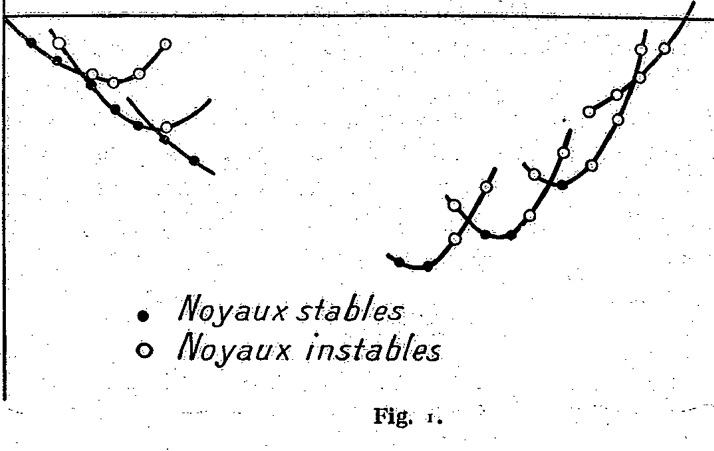
\includegraphics[width=200pt]{images/figure1}
{\caption*{Figure 1}}
\end{figure}

\subsection{Introduction of neutrons as nuclear constituents}

In the first place, on the new possibilities resulting from the discovery of the neutron by Curie and Joliot \footnote{\textsc{I. Curie} and \textsc{F. Joliot}, \textit{C. R. Acad. Sc.}, vol 194, 1932, p. 273, 876.} and by Chadwick \footnote{\textsc{J. Chadwick}, \textit{Nature}, 1932, p. 312; \textit{Proc. Roy. Soc.}, 17136, 1932, p. 692.}. This discovery is not concerned only with the existence of a particle of mass 1 and charge 0, but also shows the manner that these neutrons may figure as independent constituents of the nucleus alongside the protons and $\alpha$ particles. The experimental laws relating to spin and statistics of nuclei leading to the assumption that the neutron follows the Fermi statistics and possesses a half-integer spin. This leads to the assumption that the spin of the neutron is $\frac{1}{2}$.
Many schemas for the structure of the nucleus are compatible with this hypothesis and are obtained by introducing as nuclear constituents alongside the $\alpha$ particles and neutrons, the protons and electrons, or only the neutrons ans protons. These schemas have been discussed very completely by Perrin \footnote{\textsc{F. Perrin}, \textit{Soc. Franc. d. Physique}, vol 324, 1932, p. 96; \textit{C. R. Acad. Sc.}, vol 194, 1932, p. 343; vol 194, 1932, p. 2211; vol 195, 1932, p. 236.}, Iwanenko \footnote{\textsc{D. Iwanenko}, \textit{Nature}, vol 129, 1932, p. 312.}, Gapon \footnote{\textsc{E. Gapon}, \textit{Zeits. f. Phys.}, v. 79, 1932, p. 676; v. 81, 1933, p. 419; v. 82, 1933, p. 404; \textit{E. N. G.} and \textsc{D. Iwanenko}, \textit{Naturw.}, v. 20, 1932, p. 792.}, Bartlett \footnote{\textsc{J. Bartlett}, ??????} and Landé \footnote{\textsc{A. Landé} ?????}; it will suffice for this report to show a few selected schema exemplifying their characteristic differences. (We will here employ the symbols $\He$ = $\HeFourTwo$, proton = $\HOneOne$, neutron = $\nOneZero$, electron = $\electron$):

\begin{table}[h!]
\centering
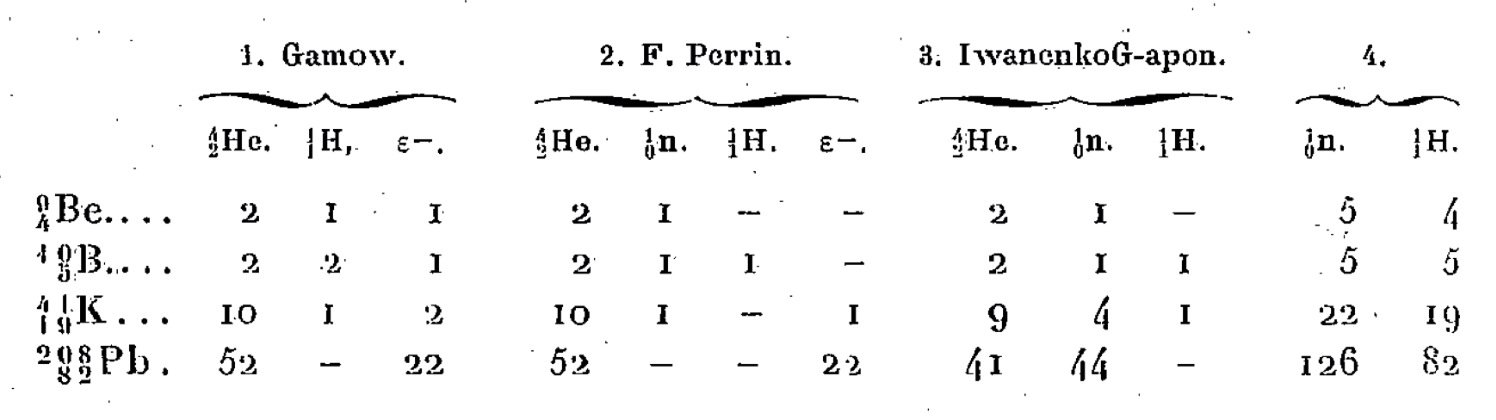
\includegraphics[width=300pt]{images/table1}
\end{table}

The last column contains a different expression than that contained in the preceding; one there considers as well the $\alpha$ particles which are composed of two neutrons and two protons. The schema of the second column considers the neutrons as elementary, non-dissociable constituents and, to take account of the $\beta$ disintegration the radioactive elements, introduced explicitly, alongside the neutrons, the electrons as nuclear constituents. Athough this conception leads to the interesting point of view on the $\beta$ radioactivity of elements, -- F. Perrin connects for example the $\beta$ of $\isotope{K}{41}{19}$ with the first appearance of a nuclear electron (c.f. Table I) -- it raises the same objections as the schema I from Gamow due to the introduction of nuclear electrons. On the contrary, the third and fourth conceptions interpreting the empirical laws concerning the spin and statistics of nuclei by making an appeal to the simple properties of neutrons, but faces difficulties concerning the $\beta$ activity; in fact, we must admit in the third and fourth conceptions that the neutron may, in favorable circumstances, decompose itself into a proton and an electron. It is true that, even in this hypothesis, it is difficult to give a precise meaning to the assertion that a neutron is composed of an electron and a proton, because it could lead, in the literal interpretation, to inaccurate conclusions concerning the spin and statistics of the neutron; in addition, the neutron experimentally manifests a strong stability much larger than would seem to result from their mass defect with respect to the combination of a proton and a neutron (this neutron mass defect is, after Chadwick, is in the environment of 1 to 3 million electron-volts, while in the disintegration of $\isotope{Be}{9}{4}$ the neutrons are driven from the nucleus with energies ranging from 8 million electron-volts. F. Perrin, in his report for the Leningrad Congress, issued a credible hypothesis for the appearance of a $\beta$ particle in $\beta$ disintegration must be accompanied by the production of a pair of positive and negative electrons along with a $\gamma$ quantum (c.f. Joliot's report), and which, consequently, in favorable energetic conditions, one may have in addition to the decomposition of a neutron into a proton and a negative electron a proton into a neutron and a positive electron. Although this hypothesis remains without a precise theoretical base, it seems possible to reconcile the stability of the neutron and of the proton with the experimental fact of the $\beta$ disintegration of certain elements. If one considers the preceding difficulties as necessary consequences of the impossibility of applying the quantum mechanics to electrons in the nucleus, the schemas 3 and 4 seem to present over 1 and 2 the advantage of making clear the limits of applicability of quantum mechanics. The schemas 3 and 4 bring into evidence the fact that the current theories do not permit one to approach the question of mutual actions between neutrons and protons, thus the problem of $\beta$ activity. On the other hand, if one introduces a law of action determined between neutrons and protons, the question of the structure of the nucleus may be studied completely by the application of the laws of quantum mechanics. Although the conceptions 3-4 are barely better justified by experiment than the first two, it seems useful to develop the consequences of the application of the quantum mechanics.
\subsection{The laws of mutual action}
The mutual action between protons and neutrons may, whether it is envisaged as an ordinary force, or, by analogy with the case of molecules, be considered as an exchange action; the first hypothesis corresponds to the idea of an elementary, indissociabld neutron, whereas the second is applied in a natural way with schemas 3 and 4. Varioua other hypotheses are also possible to describe this exchange action. One may first of all admit an analogy as close as possible between the mutual proton-neutron action and that which intervenes between the molecules $\bond{\H}{\Hplus}$. The action in this case that of an exchange action where the negative charge passes from one particle to another without modifying eachothers' spin. On the contrary, one may start from the most important experimental laws concerning the nucleus and see which exchange interactions permit taking account as accurately as possible (?.????). Majorana has shown that one thus leads to a type of action wherein the negative charge and the spin are simultaneously exchanged between the particles. We will further examine the mathematicak expression of this conception.
Various hypotheses are equally possible as concerns the mutual interaction of neutrons. It seems besides that this action between neutrons in the nucleus are much smaller than between a neutron and a proton, such that one obtains a reasonable approximation to reality by initially ignoring them completely.
By introducing this hypothesis and assuming also that, in the light nuclei, the Coulomb forces between protons being likewise ignored in the first approximation, one obtains the following results: for a nucleus of a given mass, the condition most favorable to energetic stability is equal numbers of protons and neutrons (thus resukys from the symmetry in this problem with respect to neutrons and protons). For the heavy nuclei, the electric repulsion of the protons displaces the configuration of minimal energy by a smaller number of protons and a greater number of neutrons. The fact that these results are in good accord with the experimental data relative to nuclei provides, inversely, an argument in favor of the hypothesis that the mutual neutron-neutron interaction is much weaker than that of a neutron on a proton.
The mathematical representation of the exchange action may develop in two different manners.
\begin{enumerate}
    \item One may introduce for each nuclear particle five coordinates: three for the position $\vrk$ one for the spin $\spink$, and one variable $\rhok$ which takes the value +1 or -1 following whether the particle is a neutron or a proton;
    \item Each particle is characterized by four variables: $\vrk$ abd $\spink$, but the coordinates will be designated in a different manner for neutrons and protons (e.g. $\vrK$, $\spinK$ and $\vrk$, $\spink$).
\end{enumerate}

The Schrödinger function is described thus: in the first case

\uequ{
\psi(\vrX{1}, \spinX{1}, \rhoX{1}; \vrX{2}, \spinX{2}, \rhoX{2}, ...)
}

and in the second

\uequ{
\psi(\vrX{I}, \spinX{I}; \vrX{II}, \spinX{II}; ... \vrX{1}, \spinX{1}; \vrX{2}, \spinX{2}; ... )
}

The relations between the two schemas are expressed by the equations

\nequ{
\begin{split}
\psi(\vrX{1}, \spinX{1}, +1; \vrX{2}, \spinX{2}, +1, ...) &= \psi(\vrX{I}, \spinX{I}; \vrX{II}, \spinX{II}; ...),\\
\psi(\vrX{1}, \spinX{1}, -1; \vrX{2}, \spinX{2}, +1, ...) &= \psi(\vrX{I}, \spinX{I}; \vrX{1}, \spinX{1}; ...),\\
\psi(\vrX{1}, \spinX{1}, -1; \vrX{2}, \spinX{2}, -1, ...) &= \psi(\vrX{1}, \spinX{1}; \vrX{2}, \spinX{2}; ...),
\end{split}
}{9}

If one introduces the matrices:

\uequ{
\isox = \begin{vmatrix}
 0 & 1\\
 1 & 0
\end{vmatrix};
\isoy = \begin{vmatrix}
0 & -i\\
i & 0
\end{vmatrix},
}

the mutual action term in the Hamiltonian function under the hypothesis of a simple exchange of negative charge (figure 2)

\begin{figure}[h!]
\centering
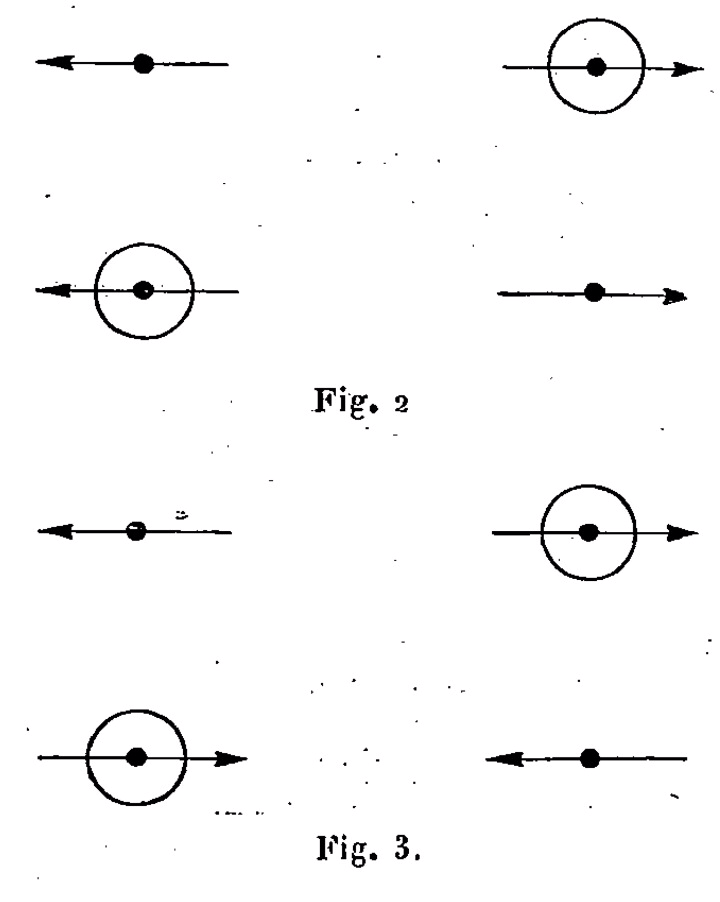
\includegraphics[width=200pt]{images/Fig2Fig3}
\end{figure}

and with the first representation becomes:
\nequ{
\XJ(\rkl)\frac{1}{2}\left[ \isokx\isolx + \isoky\isoly \right]
}{10}

or, in the second representation:

\nequ{
-\XJ(\rKl)\PprimeKl
}{11}

where $\PprimeKl$ represents the permutation operator of the variables $\vrK$, $\spinK$, with $\vrX{l}$ $\spinX{l}$.
The exchange action introduced by Majorana which will be discussed later (which is represented schematically in figure 3) leads on the contrary to the Hamiltonian in the terms which are written in the first representation:

\nequ{
\XJ(\rkl)\frac{1}{4}\left[ \isokx\isolx + \isoky\isoly \right]\left[ 1 + (\spink\spinl) \right],
}{12}

and in the second representation:

\nequ{
-\XJ(\rKl)\PKl
}{13}

where $\PKl$ is the operator corresponding to the permutation of spacial coordinates $\vrK$ and $\vrl$.
To reduce the number of possible hypotheses for exchange action, Majorana \footnote{\textsc{E. Majorana}, \textsc{Zeits. f. Phys.}, v. 82, 1933, p. 137} appealed to those that most simply fit the experimental facts. One of the most characteristic traits of the nuclear structure consists in that the nuclear radius seems to vary as the cubic root of the mass (see section 2a), that is to say that the density of nuclear matter appears to be sensibly independent of the magnitude thereof. This seems to suggest that the nucleus is not, as opposed to the atom itself, a central system within which a particular point acts as a center of force, but on the contrary, presents an analogy with the liquid state, as we have noted regarding Gamow's "blob" model, where the size of the blob is not influenced by the conditions which are present alongside of a new molecule (???). The theory of liquids shows that the existence of a finite molecular radius and the presence of mutual actions of the Van der Waals type constitute the essential bases of a representation of the state of the liquid. in the same manner, the experimental properties of the nucleus can be represented in the hypothesis of ordinary forces between protons and neutrons only if one introduces a finite radius for the neutron, that is to say a minimum distance beneath which appears an important repulsive force between the proton and the neutron. this consequence, rather difficult to accept, may be avoided by the introduction of an exchange action between protons and neutrons. In fact, as shown in the theory of Heitler and London, these exchange actions give rise to a saturation in the bonds, which leads to results analogous with the hypothesis of a finite neutron radius. One such saturation intervenes when the sign of $\J(\rKl)$ in equations (10) and (13) is positive. One will find further mathematical development below.
Majorana legitimately draws the conclusion, -- in opposition with a previous hypothesis in this report -- which, for reasons of experimental order, the positive sign is the most likely for $\J(\rKl)$. An additional argument in favor of the conception (12) and (13) against (10) and (11) resulta from the fact that in this previous conception the nucleus $\isotope{H}{1}{2}$ already represents a closed system, while under the action of forces reprrsented by (12) and (13) this saturation appears only in the nucleus of Helium.
We now indicate the mathematical justification for these results. Following the example of Majorana, we will apply to a composite nucleus with a large number of particles the Thomas-Fermi method in the formngiven by Dirac. We will choose, will Majorana, the second of the representations on page 301 (translator: the form without isospin). In these conditions, the Schrödinger function, for a nucleus composed of $\numNeutrons$ neutrons and $\numProtons$ protons, may have, in the be put (in the first approximation) in the form


\uequ{
\aWF = \begin{vmatrix}
 \WFxy{1}{I} & ... & \WFxy{\numNeutrons}{I} \\
 \WFxy{1}{II} & ... & \WFxy{\numNeutrons}{II} \\
        ... & ... & ... \\
 \WFxy{1}{\numNeutrons} & ... & \WFxy{\numNeutrons}{\numNeutrons}
\end{vmatrix}\begin{vmatrix}
\WFxy{1}{1} & ... & \WFxy{\numProtons}{1} \\
 \WFxy{1}{2} & ... & \WFxy{\numProtons}{2} \\
        ... & ... & ... \\
 \WFxy{1}{\numProtons} & ... & \WFxy{\numProtons}{\numProtons}
\end{vmatrix}.
}

The total potential energy corresponding to $\aWF$ for the exchange actions (13) becomes:

\newcommand{\opCC}[1]{{#1}^{*}}
\nc{\rKk}{\var{r}_{K,k}}
\nc{\PKk}{\var{P}_{K,k}}
\nc{\sig}{\comp{\sigma}}
\nc{\sigp}{\comp{\primed{\sigma}}}
\newcommand{\chiX}[1]{\var{\chi}_{#1}}
\newcommand{\CCchiX}[1]{\opCC{\var{\chi}}_{#1}}

\nc{\chik}{\chiX{k}}
\nc{\chiK}{\chiX{K}}
\nc{\CCchik}{\CCchiX{k}}
\nc{\CCchiK}{\CCchiX{K}}


\nequ{
\begin{split}
\Epot =& \int{\opCC{\aWF}\ser{K,k}{\XJ(\rKk)\PKk\aWF}d\omega} \\
    =& \ser{\sig\sigp}{
      \int{\int{d\vr d\vrp
        \serXY{K=1}{\numNeutrons}{
          \opCC{\WF}_{K}(\vr, \sig)\WF_{K}(\vrp, \sig)
        }\times\serXY{k=1}{\numProtons}{
         \opCC{\WF}_{k}(\vrp, \sigp)\WF(\vrp,\sigp)\XJ(\vr -\vrp)
        }
      }}
    }
\end{split}
}{15}

If one ignores the actions exerted by the particles' spin and if one consequently writes $\WF_{K}(\vr,\sig)$ as $\chiK(\vr)\var{f}_{K}(\sig)$ then equation (15) takes the form

\nequ{
\Epot = -\int{\int{d\vr d\vrp
  \serXY{K=1}{\numNeutrons}{
    \CCchiK(\vr)\chiK(\vrp)\XJ(|\vr - \vrp|)
  }
  \serXY{k=1}{\numProtons}{
    \CCchik(\vrp)\chik(\vr)
  }
}}.
}{16}

The expressions

\nc{\isoN}{\isoX{N}}
\nc{\isoP}{\isoX{P}}
\nc{\vp}{\vect{p}}
\nc{\vpp}{\primed{\vp}}
\nc{\pN}{\var{p}_{\comp{N}}}
\nc{\pP}{\var{p}_{\comp{P}}}
\nc{\pNr}{\pN(\vr)}
\nc{\pPr}{\pP(\vr)}
\nc{\rhoN}{{{\var{\rho}}_{N}}}
\nc{\rhoP}{{{\var{\rho}}_{P}}}
\nc{\rhoNrrp}{\rhoN(\vr, \vrp)}
\nc{\rhoPrrp}{\rhoP(\vr, \vrp)}
\nc{\midrrp}{\frac{\vr + \vrp}{2}}
\nc{\diffrrp}{\vr - \vrp}
\nc{\vs}{\vect{s}}
\nc{\s}{\var{s}}
\nc{\dvr}{d\vr}
\nc{\dvrp}{d\vrp}
\nc{\dvs}{d\vs}
\nc{\dvp}{d\vp}
\nc{\dvpp}{d\vpp}
\rc{\i}{\const{i}}
\nc{\f}{\var{f}}
\nc{\fivethirds}{{\frac{5}{3}}}
\nc{\cone}{\const{c_1}}
\nc{\ctwo}{\const{c_2}}
\nc{\V}{\const{V}}

\renewcommand{\exp}[1]{{\const{e}^{#1}}}
%\newcommand{\exp}[1]{{\const{e}^{#1}}}

\nequ{
\begin{split}
   \isoN(\vr) &= \serXY{K=1}{\numNeutrons}{\CCchiK\chiK} \\
   \isoP(\vr) &= \serXY{k=1}{\numProtons}{\CCchik\chik}
\end{split}
}{17}

which represents respectively the density of neutrons and that of protons replaced, as we know, in the Thomas-Fermi method by

\nequ{
  \isoN(\vr) = \frac{2}{\hbar^3}\intXY{0}{\pNr}{d\vp},
  \isoP(\vr) = \frac{2}{\hbar^3}\intXY{0}{\pPr}{d\vp}
}{18}

where the limits $\pN$ and $\pP$ are determined by fhe potential energy at the point $\r$. In an analogous manner, one writes (with Dirac \footnote{\textsc{P.A.M. Dirac}, \textit{Proc. Cambr. Phil. Soc.}, v. 26, 1930, p. 376.}):

\nequ{
\begin{split}
\serXY{K=1}{\numNeutrons}{
  \CCchiK(\vr)\chiK(\vrp) 
} = & \rhoNrrp = \frac{2}{\hbar^3}\intXY{0}{\pN(\midrrp)}{
  d\vp\exp{\frac{\const{i}}{\hbar}\vp(\vrp - \vr)}
}, \\
& = \rhoPrrp = \frac{2}{\hbar^3}\intXY{0}{\pP(\midrrp)}{
  d\vp\exp{\frac{\const{i}}{\hbar}\vp(\vrp - \vr)}
},
\end{split}
}{19}

from which it follows

\nequ{
  \Epot = -\int\int d\vr d\vrp \frac{4}{\hbar^6}\intXY{0}{\pN}{
    d\vp\intXY{0}{\pP}{d\vpp}{
      \exp{\frac{\const{i}}{\hbar}(\vp - \vpp)(\vr - \vrp)}
      \XJ(|\vrp - \vr|)
    }
  }.
}{20}

As indeed $\rhoNrrp$ and $\rhoPrrp$ only differ from zero in a small interval around $(\vrp - \vr) = 0$ or when the particle density is large, and since, on the other hand, for most nuclei $\pN > \pP$, that is to say $\rhoN > \rhoP$, one may give (20) the following form if $\J(|\vrp - \vr|)$ varies regularly with $|\vrp - \vr|$ and more slowly than $\rhoNrrp$ in the neighborhood of the point $(\vr - \vrp) =0$:

\nequ{
\Epot \approx -2\int d\vr \var{\rho}(\vr)\XJ(0) = -2\numProtons\XJ(0).
}{21}

This gross approximation is not however sufficient for the determination of $\rhoN$ and $\rhoP$ in a given nucleus. To obtain a better approximation, one may, by grace of the rapid variation of $\rhoNrrp$ with $(\vr - \vrp)$, replace the equation (20) with

\nequ{
\begin{split}
\Epot \approx & -\int \dvr \int \dvs \frac{4}{\hbar^6}\intXY{0}{\rhoN(\r)}{
  \dvp\intXY{0}{\rhoP(\r)}{
    \dvpp \exp{\frac{\i}{\hbar}(\vp-\vpp)\vs}\XJ(|\s|)
  }
} \\
 = & -\int \dvr \f \left[ \rhoN(\vr), \rhoP(\vr) \right],
\end{split}
}{$21^a$}

where $\f$ is a function that is symmetrical in $\rhoN$ and $\rhoP$, which vanishes with $\rhoN$ or $\rhoP$ and which tends, for large densities, to the limits $2\rhoN\J(0)$ or $2\rhoP\J(0)$ following whether $\rhoN < \rhoP$ or $\rhoP > \rhoN$.
Since the other part of the kinetic energy, according to Thomas and Fermi, is given by

\uequ{
\Ekin = \frac{\hbar^2}{\M}\frac{4\pi}{5}\left( \frac{3}{8\pi} \right)^{\fivethirds}
\int \dvr(\rhoN^{\fivethirds} + \rhoP^{\fivethirds}),
}

which results in

\nequ{
\E = \int \dvr \left[ \frac{\hbar^2}{\M}\left(\frac{4\pi}{5}\right)^{\fivethirds}
   (\rhoN^{\fivethirds} + \rhoP^{\fivethirds}) \f(\rhoN, \rhoP) \right].
}{22}

One obtains the functions $\rhoN(\vr)$ and $\rhoP(\vr)$ by varying $\rhoN$ or $\rhoP$ in $\E$ under the conditions:

\nequ{
\numNeutrons = \int\rhoN\dvr, \int\rhoP\dvr
}{23}

which results in

\uequ{
\rhoN(\vr) = \text{const.} = \cone, \rhoP(\vr) = \text{const.} = \ctwo
}.

If $\V$ is the volume of the nucleus, one has

\uequ{
\cone = \frac{\numNeutrons}{\V}, \ctwo = \frac{\numNeutrons}{\V}
}

and therefore

\nequ{
\E = \frac{\hbar^2}{\M}\frac{4\pi}{5}\left( \frac{3}{8\pi} \right)^\fivethirds
(\numNeutrons^\fivethirds + \numProtons^\fivethirds)\V^{-\frac{2}{3}} 
  - \V\f(\frac{\numNeutrons}{\V}, \frac{\numProtons}{\V})
}{24}

and the result of $\dXdY{\E}{\V} = 0$:

\nequ{
\begin{split}
&-\frac{\hbar^2}{\M}\frac{8\pi}{15} \left( \frac{3}{8\pi} \right)^\fivethirds\left[ 
\left( \frac{\numNeutrons}{\V} \right)^\fivethirds +
\left( \frac{\numProtons}{\V} \right)^\fivethirds
\right] \\
&-\f(\frac{\numNeutrons}{\V}, \frac{\numProtons}{\V}) + \frac{\numNeutrons}{\V}\pdXdY{\f}{\rhoN}
+ \frac{\numProtons}{\V}\pdXdY{\f}{\rhoP} = 0,
\end{split}
}{25}

the condition which determines the volume of the nucleus. If the ratio $\frac{\numNeutrons}{\numProtons}$ is held constant, the result of (25) is that the volume of the nucleus varies proportionally to the mass. This demonstrates that the exchange actions introduced by Majorana, leading, for the nuclear matter, to characteristics analogous to those of a liquid. The rest of the saturation described above for the bonding forces result again from equation (21) according to which the exchange action of a proton can only be exerted by the medium of two neutrons.
One can see from this result why the helium nucleus appears as closed system. By virtue of the Pauli principle there is no place in the same state for two protons or two neutrons. The neutrons in a well-defined state may bind with a proton, the total binding energy being simply proportional to their number. The neutrons in other states don't contribute anything on average to the binding energy. If one imagines the nuclei constructed by successive contributions of neutrons and of protons, a new closed system must be constituted each time that two new protons and two new neutrons have been added, which may be considered as corresponding to the formation of a new helium particle.
If one had made use of the exchange actions represented by (10), (11) instead of (12),(13), one will obtain (with Majorana) instead of (15), the expression:

\nequ{
\begin{split}
\E &= -\ser{\sig\sigp}{
  \int\int\dvr\dvrp
    \serXY{K=1}{\numNeutrons}{
      \CCchiK(\vr, \sig)\chiK(\vrp, \sigp)
      \XJ(|\vr - \vrp|)
    }
    \serXY{k=1}{\numProtons}{
      \CCchik(\vrp, \sigp)
      \chik(\vr, \sig)
    }
} \\
&= -\frac{1}{2}
  \int\int\dvr\dvrp
    \serXY{K=1}{\numNeutrons}{
      \CCchiK(\vr)\chiK(\vrp)
      \XJ(|\vr - \vrp|)
    }
    \serXY{k=1}{\numProtons}{
      \CCchik(\vrp)
      \chik(\vr)
    }.
\end{split}
}{26}

The average binding energy per proton will therefore be less than half than with the actions (12), (13). For the binding forces (10), (11) the isotope $\HTwoOne$ again represents a closed system, where the neutrons must thus coincide from the point of view of their positions and their spins so that their binding energies with a proton are additive.
To calculate the mass degect corresponding to a given action law $\J(\r)$, the statistical method utilized by Majorana is not the most appropriate, because the average nuclear density is conserved, even for large values $\numNeutrons$ and $numProtons$; the errors with the statistical method consequently remain about the same for small and for large values of $\numNeutrons$ and $\numProtons$. One may however obtain a better approximation by calculating first of all by an approximate method the eigenfunction of the $\alpha$ particle via the Schrödinger equation, and in deducing the average mutual action between the $\alpha$ particles, together with the action between these particles and the protons or the neutrons. One could then apply the statistical method to a system composed of neutrons and of $\alpha$ particles and thus realize an improvement over the method described until now.

Despite the insufficiency of the method which we have just indicated, one may try to deduce, in a qualitative manner, the variation of the mass defect with $\J(\r)$, $\numNeutrons$ and $\numProtons$. It may be used, in view of the subsequent application, to pursue the consequences of a particularly simple hypothesis on the form of $\J(\r)$ and to calculate the corresponding form of the function $\f(\rhoN, \rhoP)$.
In the form proposed by Majorana
\nequ{
\XJ(\r) = \a\exp{-\b\r}
}{27}

correspond following (21):

\nequ{
\begin{split}
\f(\rhoN, \rhoP) = \a\frac{\b^3}{6\pi^3} \{
4\N\P + \lbrack 1 &+ 3(\N^2 + \P^2) \rbrack \log{\frac{1 + (\N - \P)^2}{1 + (\N + \P)^2}} \\
 &+ 4(\N^2 + \P^2)\arctan{(\N + \P)} \\
 &- 4(\N^2 - \P^2)\arctan{(\N + \P)}
\} ,
\end{split}
}{28}

where one puts

\uequ{
\N = \frac{1}{\b}\sqrt[3]{3\rhoN\pi^2} \text{ and } 
\P = \frac{1}{\b}\sqrt[3]{3\rhoP\pi^2}.
}

It follows that $\a$ is 

\uequ{
\ll \frac{\hbar^2\b^2}{\M} \text{ or } \gg \frac{\hbar^2\b^2}{\M},
}

one will have, by (25),

\uequ{
\N \text{ and } \P \ll 1 \text{ or } \gg 1.
}

Because the statistical method gives usable results, it is as a consequence necessary to suppose

\uequ{
\a \gg \frac{\hbar^2\b^2}{\M}.
}

If this condition is fulfilled, one may approximately replace the expression (28) by

\nequ{
\begin{split}
\f = \a\frac{\b^3}{3\pi^3}\{
&\pi(\N^3 + \P^3) - 2(\N - \P)^2 \\
&-\frac{3}{2}(\N^2 + \P^2)\log{\frac{(\N + \P)^2}{1 + (\N - \P)^2}} \\
&-2(\N^3 - \P^3)\arctan{(\N-\P)}
\}.
\end{split}
}{29}

These calculations must be modified in the case of heavy nuclei to take account of the Coulomb force. In place of (22) one obtains the equation

\nequ{
\begin{split}
\E = & \int \dvr \{
\frac{\hbar^2}{\M}\frac{4\pi}{5}\left(\frac{3}{8\pi}\right)^\frac{5}{3}(\rhoN^\fivethirds + \rhoP^\fivethirds) - \f(\rhoN, \rhoP)\} \\
& + \frac{1}{2} \int\int\dvr\dvrp \frac{\e^2}{|\r - \rp|}\rhoP(\vr)\rhoP(\vrp).
\end{split}
}{30}

By varying $\rhoN$ and $\rhoP$ in $\E$ one obtains equations which are transformed with the ordinary Thomas-Fermi methods into differential equations for $\rhoN$ and $\rhoP$. Under the influence of the Coulomb forces, the densities $\rhoN$ and $\rhoP$ varying in the interior of the nucleus, these Coulomb forces tend to accumulate the positive charge on the exterior surface. So long as thes forces remain weak, that is to say for not-too-large nuclei, we may treat their actions as small perturbations, and to calculate the mass defect introduce the unperturbed densities in the complementary term of equation (30).

The Coulomb energy term thus becomes:

\nequ{
\int\int \dvr\dvrp\frac{\e^2}{|\vr - \vrp|}\rhoP(\vr)\rhoP(\vrp) = \frac{3}{5}(\numProtons\e)^2
\left( \frac{3\V}{4\pi} \right)^{-\frac{1}{3}}.
}{31}

In the following chapter we will compare the formulae thus obtained with the experimental data.

\subsection{General consequences for for the table of isotopes}

The hypotheses for the structure of the nucleus, which have been developed in parts \textit{a} through \textit{c} of section two, permit us to deduce certain general conclusions about the peculiarities of the table of isotopes and about the laws of radioactive disintegration.
The diverse conceptions all lead to the result that the nuclear properties, such as stability, abundance in nature, spin, etc., present a certain periodicity for a variation 4 of the mass and 2 of the charge, which fits well with experience. The Gamow model and the schema 2 lead in particular to a very remarkable influence of the mass on the properties of the nucleus, following which this mass is of the form $4n, 4n + 1, 4n + 2 or 4n + 3$. On the contrary, the charge of the nucleus for a given mass and in particular the fact that this charge is odd or even, does not seem to play an important role. Insofar as one may speak of the properties of nuclear electrons, experience seems to indicate that they follow Bose statistics; one consequently would not expect a variation with period 2 in the charge. If on the other hand one considers the nucleus as composed of neutrons and of protons (schemas 3 and 4),one must expect in the first place a periodicity in the nuclear properties for a variation of 2 in the charge, since one always has in the presence of at least as many neutrons as protons and it always suffices that two new elementary charges for the formation of an $\alpha$ particle; in the second place for a given charge a rather less remarkable periodicity for the variation 2 of the mass by application of the Paili principle for the proton and the neutron. In the sense of the periodicity specified by the schemas 3 and 4, one must expect for example the analogies between the nuclei (???? Swap the args ?.?.????) $\isotope{Xe}{124}{54}$, $\isotope{Xe}{126}{54}$, $\isotope{Xe}{128}{54}$, $\isotope{Xe}{130}{54}$ and $\isotope{Xe}{132}{54}$ 

\begin{figure}[h!]
\centering
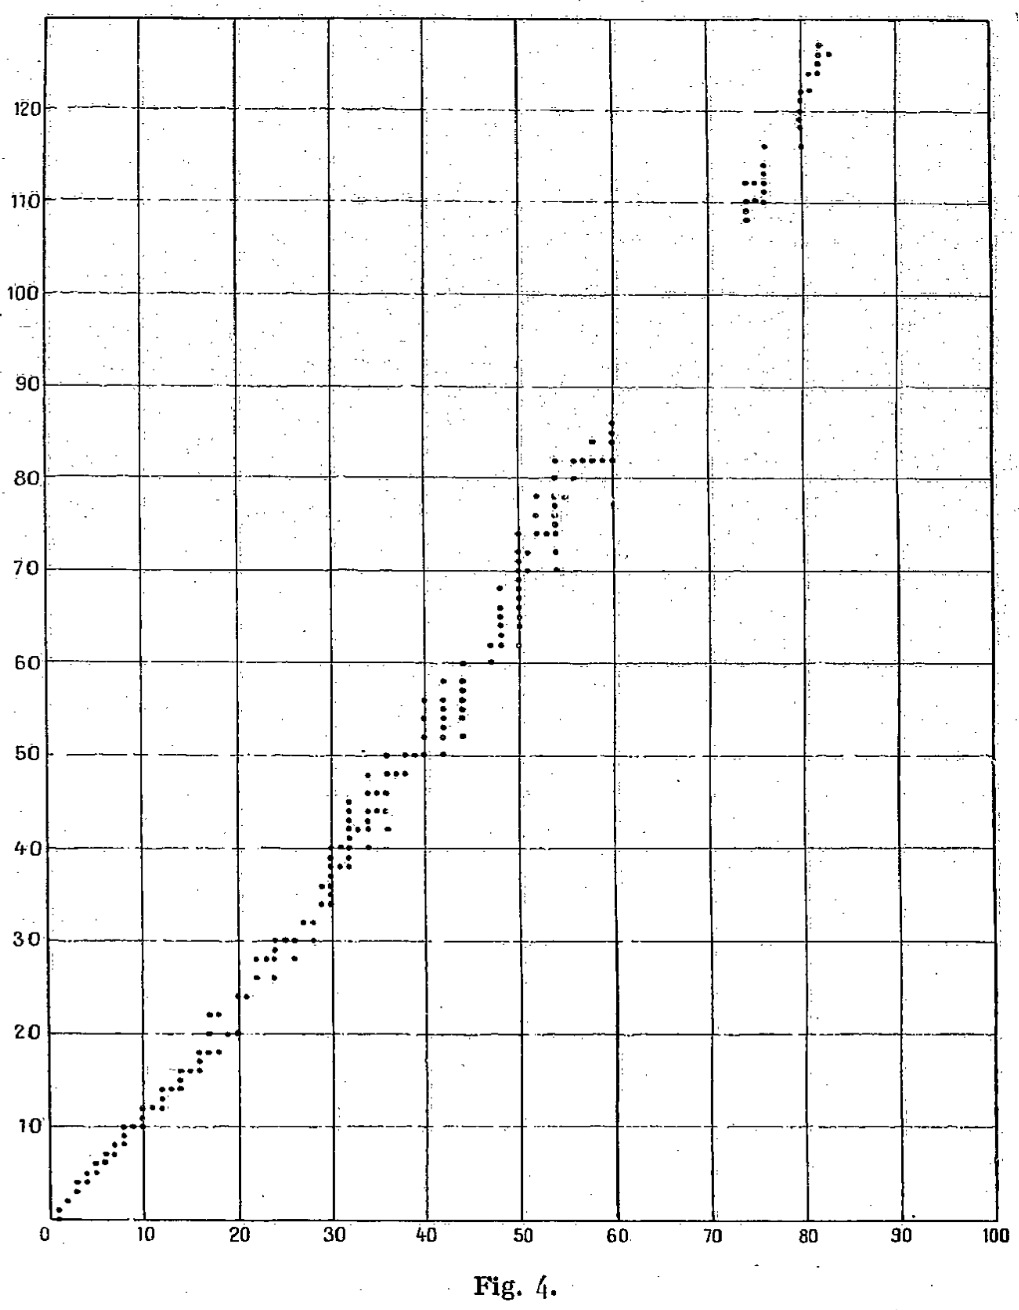
\includegraphics[width=250pt]{images/fig4}
{\caption*{Figure 4}}
\end{figure}
 whereas the periodicity which results from Gamow's scheme should provide for the nuclei $\isotope{Xe}{124}{54}$, $\isotope{Xe}{128}{54}$, and $\isotope{Xe}{132}{54}$ common characteristics whicn don't appear in the nuclei $\isotope{Xe}{126}{54}$ and $\isotope{Xe}{130}{54}$. In figure 4 the known nuclei are represented with the number of protons $\numProtons$ on the $\var{x}$ axis and on the $\var{y}$ axis the number of neutrons $\numNeutrons$, so that a point corresponds to each nucleus. The table thus clearly indicates a predominance of even charges and, less markedly, a predominance of even numbers of neutrons. This finding, although not in contradiction with Gamow's scheme, provides an argument in favor of hypotheses 3 or 4 because it may be explained by these hypotheses.

\begin{figure}[h!]
\centering
\includegraphics[width=300pt]{images/fig5}
{\caption*{Figure 5}}
\end{figure}

In this conception, one may represent in the following manner the construction of a nucleus from neutrons and protons: each time that two protons and two neutrons have been added, a new shell is completed by the formation of a Helium nucleus. For the nuclei which only contain $\alpha$ particles, there is no need to admit any shell formation beyond this Helium nucleus; in fact, the large formation energy of the $\alpha$ particles permits the consideration to a certain extent as constituent elements of the nucleus, and the fact that they follow Bose statistics results in the fact that they all tend to the lowest energy level. It is otherwise, as Landé \footnote{\textsc{A. Landé}, \textit{Phys. Rev.}, v. 43, 1933, p. 620 and 624.} justifiably insists, for the neutrons which don't enter into the constitution of $\alpha$ particles. If one admits the construction of the nucleus from $\alpha$ particles, neutrons, and eventually a proton, allows us to obtain a good approximation for the solution of the aleady-complicated problem kf the quantum mechanics of heavy nuclei, one may compare the movement of neutrons in the $\alpha$ particles' field of action with that of the peripheral electrons which surround the nucleus of the atom and therefore we expect a structure of successive shells of this system of neutrons. Landé has represented in figure 5 the experimentak number of neutrons independent of $\alpha$ particles for the different atomic numbers, and he considers that this figure leads immediately to the following interpretation: up to the charge $\numProtons = 16$, only the lowest level of a system of neutrons is occupied and may constitute a shell of two neutrons; between $\numProtons = 17$ and $\numProtons = 28$ this shell must always be çomplete and a further shell of four neutrons may be completed; from $\numNeutrons = 32$ up to $\numNeutrons = 36$ a further shell of eight neutrons will be completed, and so on. If one tries on the other hand to predict theoretically this formation of successive layers, one must first of all examine the possible stationary states of the field inside the nucleus. The distribution of potential which determines the movement of a neutron inside the nucleus is known qualitatively. The density of $\alpha$ particles should be approximately constant inside the nucleus with a small increase towards the surface because of the Coulomb forces. 

\begin{figure}[h!]
\centering
\includegraphics[width=300pt]{images/fig6}
{\caption*{Figure 6}}
\end{figure}

This results for the neutron in a variation in potential of the form represented in figure 6. The states of weaker energy which correspond to this potential represent, if one ignores the reaction of spin on the orbital angular momentum, a term $\orbit{S}(\l=0)$, a term $\orbit{P}(l=1)$, and a term $\orbit{D}(l=2)$ (cf. Gamow's report, figure 10). If one brings in a hypothesis a involving spin interaction, one will obtain for the lowest terms a schema analogous to that in figure 7. Besides this schema, one will get firstof all a shell of two, and then one of four neutrons (appearing in the term $\j = \frac{3}{2}$), and again a shell of two, one of six, one of four, etc. It is not yet possible to grasp the extent to which a similar schema constructed from individual neutron orbits can account for the experimental facts concerning the system of isotopes.

\begin{figure}[h!]
\centering
\includegraphics[width=300pt]{images/fig7}
{\caption*{Figure 7}}
\end{figure}



The question of the stability of the nucleus from the point of view of $\alpha$ disintegration is completely elucidated by the theory of Gamow, Condon and Gurney (cf. Gamow's report); the Gamow theory is also applicable in a manner analogous to diverse nuclear models. Since this theory depends on the stability of the nucleus with respect to $\alpha$ disintegration, only the energy balance of this process, one may admit that, for a given nuclear mass, the Coulomb forces make the disintegration much more probable when the nuclear charge is larger. The fact that there exists experimentally, for a given mass, an upper limit on the charge far below the atomic weight, leads naturally to the hypothesis that nuclei of high charge dissociate with the emission of $\alpha$ particles. One also finds that, among the radioactive nuclei of the same mass, it is generally those with the highest charge that manifest the largest disintegration energy.
It is currently difficult to treat in a satisfactory manner the question of nuclear stability with respect to $\beta$ disintegration. In the primitive theory of Gamow, the energy balance determines the stability from the point of view of the emission of a $\beta$ ray as well as that of $\alpha$ rays. This conception is not simply justified, because it is an experimental fact that the $\beta$ particles emitted from the nucleus follow a continuous energy spectrum, and because there does not sedm to be a relationship between the average $\beta$ decay energy and the mean lifetime, which is analogous to that of Geiger-Nuttall for the $\alpha$ disintegrations. However, this question remains open, because a clearly-defined upper limit of the continuous $\beta$ spectrum represents a difficulty for all theories relying upon the principle that $\beta$ particles are emitted from the nucleus with an indeterminate energy. Pauli has examined the hypothesis that $\beta$ decay is always accompanied by a very penetrating radiation consisting for example of a "neutrino" of mass equal to that of the electron, which permits the maintainence of the principle of conservation of energy and monentum in $\beta$ decay. Bohr \footnote{?????} considered on the contrary as more likely that nuclear $\beta$ decay is an exception to the principle of conservation of energy.
The theoretical aspect of this question of $\beta$ decay is not modified if we consider the nucleus as constituted from neutrons and protons. In this case, the question of stability with respecr to $\beta$ decay is reduced to knowing if a neutron can decay into a proton and an electron when it us found in an field that is energetically favorable to this decay. For the solution of this problem, we will have, for the reasons indicated above, to be content will the experimental findings. If the energy balance can determine the $\beta$ stability, there must exist an upper limit on the mass for each given nuclear charge beyond which the nucleus decays by emitting an electron. It is as a consequence used to start to establish the mass defects, insofar as they are known empirically or theoretically, the energy balance for the $\beta$ disintegration, and in comparing the results with the table of known stable nuclei. We will give the result of this comparison with the applications of Majorana's formula.
If one considers the $\beta$ decay as determined by the energy balance, the conception 3-4 gives a satisfactory interpretation of the fact that the $\beta$ emissions from a nucleus with initially even charge always come in consecutive pairs. If, in fact, the energetic conditions are favorable to the emission of a first $\beta$ particle, a second emission, after which a new $\alpha$ particle may be formed in the nucleus, for which energetic conditions will be at least as favorable \footnote{\textsc{Heisenberg}, \textit{Zeits. f. Phys.}, v. 77, 1932, p. 1; v. 78, 1932, p. 1932, p. 156; v. 80, 1933, p. 587}. It is only for an initially odd nuclear charge that a sole $\beta$ particle may eventually be emitted (Ac). The fact that there are no stable nuclei above $\isotope{N}{7}{14}$ with odd numbers of protons may in the same manner receive a simple energetic interpretation.


\section{Applications}
\subsection{Mass-defect and stability of nuclei}

One obtains very precise indications on the subject of the variation of the mass defect by starting with the hypothesis of the nuclear structure corresponding to the schemas 3-4, in particular when one takes the point of view of Majorana, which one may consider as corresponding with a form of the Gamow "blob" model clarified by the neutron hypothesis. One may try to determine the two constants of the force law introduced in $\J(\r) = \a\exp{-\b\r}$ in the matter that the mass defects of two properly chosen nuclei being exactly represented by the equation (30), and to see which way the mass defects calculated for other nuclei with this same formula are placed with respect Aston's experimental curve. In this comparison one must remember that the Thonas-Fermi metbod used to obtain equation (30) does not give exact results for light nuclei. The equation must however represent in a qualitative manner the mass defects for the various nuclei above $\n = 20$, for example, although it must give an absolute value much higher than the binding energy, because this energy, per particle, is certainly weaker for the very light nuclei than the heavy nuclei. By adding a constant term to the second part of (30), one should be able to approach the true value.
If one puts for example in $\J = \a\exp{-\b\r}$:

\uequ{
\begin{split}
\a =& \M\c^2\times 0.0273 = \ee{4.05}{-5} \text{erg},\\
\b =& \frac{\M\c}{\hbar}\times 0.165 = \ee{1.25}{12} \text{cm}^{-1}
\end{split},
}

on deduces after these calculations, from equations (30) and (31), the expression approximates:

\nequ{
\begin{split}
\frac{\E}{\M\c^2} = &0.00347\numProtons - 0.0364\numNeutrons + 0.01211\frac{\numNeutrons^2}{\numProtons}\\
&+ \numProtons^\fivethirds(3.19 - 0.715\frac{\numNeutrons}{\numProtons})\dot 10^{-4}(+0.049).
\end{split}
}{33}

The first line represents the influence of exchange actions, the second includes the action of the Coulomb repulsion between the protons and the additive term just discussed and which is not contained in equation (30); this term is chosen in a manner to retrieve the most possible of Aston's values. Figure 8 gives the results of the comparison of values thus calculated with those measured by Aston; the mass of the neutron will be, for this comparison, supposed to be equal to that of the proton.

\begin{figure}[h!]
\centering
\includegraphics[width=300pt]{images/fig8}
{\caption*{Figure 8}}
\end{figure}

One musf not attribute too much significance to the relatively good agreement which results from this comparison because, for the establishment of formula (33), one must dispose of three arbitrary constants and which, otherwise, as insited by Majoraba and as we have indicated above, the application of the Thomas-Fermi method may include important errors, even for sufficiently-large numbers of particles. One may however conclude that the formuka (30) gives, in a qualitative manner af least, the correct variation of the energie with $\numNeutrons$ and $\numProtons$. We must attach a greater importance to the consequences which may be deduced from equations (30) and (33) concerning the stability of atomic nuclei. The energy necessary to extract two protons and two neutrons from the nucleus is given by (33), in fractions of the intrinsic energy of the proton, by

\nequ{
\begin{split}
-2\left( \pdXdY{\E}{\numNeutrons} + \pdXdY{\E}{\numProtons} \right) = & 0.0658 - 
0.04844\frac{\numNeutrons}{\numProtons} + 0.02422\left( \frac{\numNeutrons}{\numProtons} \right)^2 \\
& + \left(9.2 - 0.954\frac{\numNeutrons}{\numProtons}\right)\numProtons^{\frac{2}{3}}\dot 10^{-4}.
\end{split}
}{34}

If this energy is greater than the binding energy of the helium nucleus, the nucleus being considered is stable with respect to a disintegration; if on the contrary this energy is smaller, if may spontaneously emit an $\alpha$ particle.

Figure 9 shows the constant disintegration-energy curves starting from the experimental value of the mass defect of the $\alpha$ particle and assuming for the neutron a mass defect negligably different from that of a proton and electron.

One of these curves, that which corresponds to $\Delta\E = 0$, must represent the limit between the stable and unstable atomic nuclei. If one focuses on the poibts corresponding to experimentally-stable atomic nuclei, one finds that the lower limit of these points fits well in general with the curve corresponding to null disintegration energy; the curve $\Delta\E = -0.003$ would fit better than $\Delta\E = 0$, but being given the arbitrary approximations (the mass of the neutron is equal to that of the proton, etc), this result may not be invoked against the validity of equation (30).

On may calculate in the same manner the energy difference between the initial and final states of a $\beta$ decay process:

\nequ{
\begin{split}
\pdXdY{\E}{\numNeutrons} - \pdXdY{\E}{\numProtons} = &-0.0399 + 0.02422\frac{\numNeutrons}{\numProtons} + 0.01211\left( \frac{\numNeutrons}{\numProtons} \right)^2 \\
& -\left( 6.04 - 0.477\frac{\numNeutrons}{\numProtons}\right)^2 \numProtons^{\frac{2}{3}}\dot 10^{-4}
\end{split}
}{35}

\begin{figure}[h!]
\centering
\includegraphics[width=300pt]{images/fig9}
{\caption*{Figure 9}}
\end{figure}

The curves of constant disintegration energy (figure 9) are found to be for the most part parallel to the upper limit of the poinrs corresponding to stable atomic nuclei, and and this representa an argument in favor of an energetic criterium for the stability with respect to $\beta$ emission. The curve $\Delta\E = 0$ is again found to be seemingly too low. One must therefore remark that, for for $\alpha$ decay as well as $\beta$ decay, the curve $\Delta\E = 0$ may not represent exactly the limit of experimentally-stable atomic nuclei. In fact, it is a result of Gamow's theory of disintegration that the heavy nuclei, even though they can emit an $\alpha$ particle with kinetic energy of $\ee{5}{-6}\unit{erg}$, they behave as if they are practically stable because of their long average life; analogous circumstances are probably present in the case of $\beta$ emissions \footnote{See the note at the end of this report.}.

\begin{figure}[h!]
\centering
\includegraphics[width=300pt]{images/fig10}
{\caption*{Figure 10}}
\end{figure}

Figure 9 bshows clearly why there are no stable nuclei above a certain nuclear charge determined by the intersection of the two stability curves. One must also recall that approximate methods such as the Thomas-Fermi method cannot take account of the peculiarities present in the radioactive families. To put this fact in evidence, one may compare the constant $\alpha$ decay energy curves in figure 10 in the domain of the radioactive elements tonthe experimental data. One immediately finds certain peculiarities (the maximum of the decay energy for $\primed{\element{ThC}}$) which cannot be accounted for by a superficial theory of nuclear structure. The Thomas-Fermi methos can onky give the general shape of the variation of energy.
We have so far only given a very small number of theoretical values for the mass defects of light nuclei. Wigner \footnote{\textsc{E. Wigner}, \textit{Phys. Rev.}, v. 43, 1933, p. 252} has examined to what extent the hypothesis of an ordinary action (as opposed to an exchange action) between a neutron and a proton may account for the fact that the mass defect of the isotope $\isotope{H}{1}{2}$ is fifteen times smaller than that of the helium nucleus. He found that, for a certain form of the action law, the energy of the $\isotope{H}{1}{2}$ nucleus is notably weaker in absolute value than the mean potential energy or the mean kinetic energy of the particles in this nucleus. If it is thus, the ratio of the mass defects of $\isotope{He}{2}{4}$ and $\isotope{H}{1}{2}$ becomes very large. Wigner's results may immediately extend Majorana model.

\subsection{Diffusion and disintegration}

The hypothesis that nuclei are composed of neutrons and protons and that a simple action law exists between these two sorts of particles also allows simple applications to the theory of collisions between nuclei and $\alpha$ particles, protons, and neutrons. In particular, one may easily deduce from the action law between protons and neutrons that of the diffusion of neutrons by protons; inversely the experimental results concerning this diffusion allow one to directly attain the  supposedly unknown action law. Unfortunately, the presently-availabke experimental material does not permit a precise determination of this action law. Since the theory of diffusion and that of disintegration are treated in Gamow's report, (??) we will only examine here certain points concerning the peculiarities of the neutron hypothesis.

Iwanenko \footnote{\textsc{Iwanenko}, \textit{loc. cit.}} has interpreted in the following manner, in applying the neutron hypothesis, the fact that the disintegration of beryllium under the action of $\alpha$ rays only emits neutrons and $\gamma$ rays, without any protons: the beryllium nucleus of mass 9 is composed, in the hypothesis assumed here, of two $\alpha$ particles and a neutron; while the energy of the incident $\alpha$ particle is not sufficient to disintegrate the $\alpha$ particles themselves, the nucleus cannot emit anything but the neutrons. If one follows the consequences of this conception, it predicts an emission of neutrons fromnthe bombardment of carbon by $\alpha$ particles ($\isotope{C}{6}{12}$ cannot disintegrate, but the same considerations as for $\isotope{Be}{4}{9}$ apply for the rare isotope $\isotope{C}{6}{13}$ \footnote{Transcription note: the isotope number is illegible; $\isotope{C}{6}{13}$ was chosen because it seems to be the closest analogy to $\isotope{Be}{4}{9}$, since it has one excess neutron over three full $\alpha$ particles}); it predicts on the contrary the emission of a mix of neutrons and protons from $\element{Li}$, $\element{B}$, $\element{N}$ and $\element{O}$. If one uses (with Cockroft and Walton\footnote{\textsc{Cockroft} and \textsc{Walton}, \textit{Proc. Roy. Soc., A}, v. 137, 1932, p.229.}) protons to produce the disintegrations, the radiation emitted may be composed of $\alpha$ particles and neutrons. One must in particular predict the appearance of neutrons from the heavier nuclei ($\isotope{Cl}{17}{37}$ for example) which contain surplus neutrons outside of the $\alpha$ particles.
A particularly significant result from the experiments of Cockroft and Walton \footnote{The recent research of Rutherford and Oliphant seems to show that Cockroft \& Walton's results on the disintegration of very heavy elements are due in reality to secondary effecta (cf. Cockroft's report). The considerations of Teller's which have just been alluded to retain their importance for the discussion of the decay of lighter nuclei. } shows that the protons may also produce the disintegration of heavy nuclei ($\element{Co}$, $\element{Pb}$, $\element{U}$), although with a very weak yield. This result seems incomprehensible if one considers a penetration of a proton in the nucleus as a prerequisite for decay. In fact, the probability for which a proton of energy $500,000\unit{eV}$ may penetrate into a uranium nucleus is infinitely small. Teller \footnote{I am much obliged to M. Teller for an interesting discussion on these questions.} remarked on the subject of this hypothesis of the exchange action between protons and neutrons makes possible the process by which an exchange of position between an incident proton and a nuclear neutron takes place. The neutron thus produced the hasbthe possibility of penetrating in the nucleus without having to cross Gamow's barrier due to the Coulomb forces. This results in the dimunition of the decay probability, when the atomic number increases, is not represented in the general manner by Gamow's exponential factor, and the part corresponding to the exchange actions diminishes approximately as $|\J(\rmin)|^2$, where $\rmin$ represents the distance to which the proton may approach the nucleus according to the classical theory:


\nc{\Z}{\var{Z}}

\uequ{
\frac{\Z\e^2}{\rmin} = \Ekin
}

Of then $\J(\r)$ doesn't decrease rapidly enough as the distance increases, the dimunition of probability may be much weaker than that indicated by the Gamow factor. The experimental data correspond to $\J = \a\exp{\b\r}$, $\b = \ee{1.25}{12}\unit{cm^{-1}}$, leading to a slow dimunition in $\J$ relative to the increase in $\r$. It remains doubtful that these considerations suffice for interpreting the results of Cockroft and Walton regarding the heavy nuclei.

\textsc{Note added in proofs (June 6, 1934).} -- The discovery of the radioactivity with emission of positrons (Joliot-Curie) obliges us to slightly modify the preceding considerations (p. 320). To a gross approximation, which is the basisbof equations (30) to (35), the only stable nuclei should be in fact those for which $|\pdXdY{\E}{\numNeutrons} - \pdXdY{\E}{\numProtons}| \leq \m\c^2$. The stable nuclei should be distributed as in figure 9 symmetrically on either side od the curve $\pdXdY{\E}{\numNeutrons} - \pdXdY{\E}{\numProtons} = 0$. The width of the band of stable elements on either side of this curve is not however give given by the condition $|\pdXdY{\E}{\numNeutrons} - \pdXdY{\E}{\numProtons}| \leq \m\c^2$; on the contrary, the difference in energy between nuclei of even charge and those of odd charge has the effect of giving this band, in the case of nuclei of even mass, a notably larger width than would be predicted by the above condition. One will find details on this subject in \textsc{W. Heisenberg}, \textit{loc. cit.} II.

% Uncomment the following two lines if you want to have a bibliography
%\bibliographystyle{alpha}
%\bibliography{document}

\end{document}